\documentclass[10pt]{scrreprt}
\usepackage[utf8]{inputenc}
\usepackage{amsmath}
\usepackage{amsfonts}
\usepackage{amssymb}
\usepackage{graphicx}
\author{Kim Rostgaard Christensen}
\title{Requirements as tests}
\subtitle{Automatic generation of test from structured requirements}

\begin{document}
\maketitle

\begin{abstract}
The world of software is has over the years been tainted with stories about failed projects. Almost everyone has his or her on story about a given software system, that did not solve the task, which it was designed to. This indicates; either a mismatch between requirements and solution, or simply erroneous requirement specifications.
\end{abstract}

\chapter{Introduction}

\section{Terminology}
\subsection{Three kinds of models}
Informal models for communication
Formal models, which can be used for verification -- such as Z or VDM
Meta-models that model other models, such as UML


\chapter{Case project}
This project uses the open source project ``OpenReception'' as case study. The project aims to provide a drop-in replacement for an existing system, and therefore has relatively fixed requirements.

\section{End-user experience}
The challenge in documenting requirements is, and has always been, to formulate them on a non-ambiguous form. The quantification of ambiguity tends to be difficult as well, due to the fact that requirements are usually formulated in natural languages following some rules, such as pre-defined glossary and constraints. Constraints vocabulary typically consists of should, could, may, must.

As requirements are basically constraints to your system, a subset of them may be expressed as expressions following a formality that is machine-interpretable. Vienna Development Method (VDM) and Z notation are two approaches that tries to formally describe systems on a very high level, so that model-checking can be performed on it prior to programming.

Starting from scratch, the user would be expected to initially define at least one actor and add a sequence of actions that the actor perform.




\begin{figure}
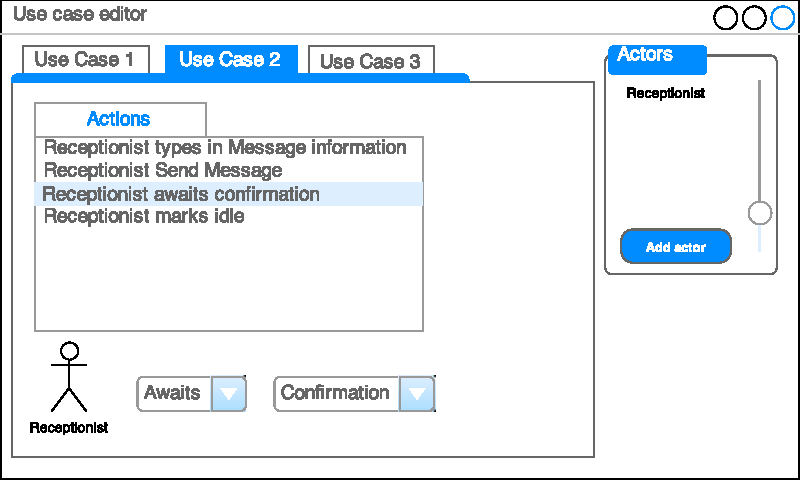
\includegraphics[scale=0.9]{img/test_case_ui}
\centering
\caption{Use case editor UI mockup}
\label{fig:use_case_editor_mockup}
\end{figure}




\section{Use case writing level}
Should not be used to describe UI actions% http://alistair.cockburn.us/Use+cases%2c+ten+years+later (Use case limits).


\section{Expressing requirements}

\section{Targeted requirements}
We've chosen to focus on the requirements that involves core features from the Receptionist actor point of view. These are, on a high level;
\begin{description}
  \item[Manage calls:] Being able to technically handle calls by performing receive, park, transfer and hangup action.
  \item[Process calls:] Being able to process calls in the context of a dialed reception. This involves having access to data about the reception and its contacts. Being able to dial them, or send them a message.
  \item[Manage message:] Being able to send out messages to contacts, view and resend existing messages.
\end{description}

This gives the following -- more detailed -- requirements
\begin{description}
  \item[RQ1: Transfer to contact:] A receptionist must be able to transfer a call to a chosen contact associated with the currently active reception. An example use case, from the receptionist actor point of view is outlined below.
  \begin{itemize}
    \item Preconditions.
    \begin{itemize}
      \item Receptionist has previously received a call $A$
      \item Receptionist has parked the previously received call $A$
    \end{itemize}
    \item Actions.
    \begin{itemize}
      \item Receptionist dials the number of the selected contact (call $B$)
      \item Receptionist hears dial tone
      \item The contact's phone is ringing.
      \item The contact accepts the calls (picks up)
      \item Receptionist has a dialogue with contact
      \item Receptionist transfers call $B$ to call $A$
      \item The system breaks the receptionist's connection to both call $A$ and $B$    
      \item Receptionist marks his/her state as idle.
    \end{itemize}
  \end{itemize}

  \item[RQ2: Send message to contact:] A receptionist must be able to send a message -- via a distribution list -- to a contact, typically containing information received verbally via a call. An example use case, from the receptionist actor point of view is outlined below.
  \begin{itemize}
    \item Preconditions.
    \begin{itemize}
      \item Receptionist may have previously received a call $A$, which may still be active.
    \end{itemize}
    \item Actions.
    \begin{itemize}
      \item Receptionist finds contact $C$ who will serve as recipient
      \item Receptionist selects $C$
      \item Receptionist types in message
      \item Receptionist sends the message via the system
      \item Receptionist marks his/her state as idle.
    \end{itemize}
  \end{itemize}
\end{description}

%TODO High leve description (customer level)

\chapter{Validating implementation}
%Something about the V-model.

\section{Formalized approaches}
%2.1. Use case description
%A semiformal use case description is simply a natural
%language text structured using a text template which divides
%the text into logical parts. Even though there is no broadly
%accepted standard use case template, the existing templates
%are quite similar.
\section{Testing}
%Fixtures
%Design by contract
%Harness

\section{Regression testing}

\chapter{Requirement formalization}
Actors, Roles

Aspects. Behavior. State space.

\section{Use case as base}
\includegraphics[scale=0.4]{img/req_meta.png}

\section{Processes}

\chapter{Test generation}
Using -- exclusively -- the use case from \textbf{RQ2} as base, we try to derive what is needed in order to generate a basic test.
To achieve the minimum implementation, we cut away the optional precondition that may be covered by other use cases. After this, we see an implicitly \emph{ordered list of actions} that we need to succeed in order for the test to be a success. There is an actor that performs an action at each step. The system, in its entirety, may also be referred to as an actor as it is also capable of performing actions.

So, summing up, we have;
\begin{itemize}
  \item This use case consists of an ordered list of actions, where actions consist of
  \begin{itemize}
	\item One or more actors
	\item One verb describing the action
	\item One target for the action (object for verb)
  \end{itemize}
\end{itemize}
If we 

\section{Requirement/test mapping}
The communication model needs to be known.

\chapter{Process evaluation}

\chapter{Conclusion}


% PROJECT DESCRIPTION BELOW.


\section*{Background}
Within software projects, documented requirements often become outdated and irrelevant over time as requirements are implemented and verified manually. For long-lived projects that continuously add features and components, maintenance of requirements becomes increasingly cumbersome, and increases the risk of requirement documentation decay further. Dynamic documents -- for instance, an inter-linked web document written in wiki markup -- may make requirement maintenance more accessible. This applies to both humans, but especially also for computers that may extract valuable information about system requirements for use in system verification tests.\\\\
Additionally, if the requirements are formalized in a sufficiently structured way, and annotated with references to the implementation, the cost of requirements maintenance may be made worthwhile by enabling us to automatically generate system tests from them.
\subsection*{Project}
The key idea is that sufficient structure in requirement formalization may enable tests to be generated directly from requirements fully automatically. To facilitate this, it means that requirements should be written with a strong focus on testability. This, as a side effect, may increase the motivation for quantifying, constraining and refining requirements. As an example: \emph{Who} will perform this action, and how are the outcomes expected to be presented/received?\\\\
The project will use the requirements from an existing system as a case study and formalize the structure of these, so that test generation from them is possible. During this process, we will investigate how to structure requirements so that we can generate tests directly from them and map implementation to requirements. Ideally, we want to identify general patterns and constraints in the structure/formalism introduced to our requirements in the case study, to be able to apply them to other projects. But in general, we will investigate to which extent this idea can be applied.
%In the software engineering field, a paradigm shift from waterfall-oriented development methods, towards more agile and iterative methods. However, the iterative approach still has a requirements phase, that may play an only minor role in the implementation phase, and focus shifts to \emph{how to make it work}, rather than \emph{what it should do}. Test-driven development handles this pragmatically by enforcing that tests are written before implementations. This provides a strong interface-driven black-box oriented methodology. It also provides a feedback channel for requirement changes.\\\\
%Taking test-driven development a step further, one may perceive the software system in its entirety as a large interface, and it's requirements as the tests. Use cases are textual descriptions of the functional requirements of the system, which are typically written in a semi-formal language, using only terms clearly defined within a domain model or glossary.\\
%Applying transformations to use cases derived from requirements, turning them into automated acceptance tests, could provide a more requirement-oriented development method, keeping the requirements in the loop during the entire development process.

%\section{Project}
%The approach motioned above is influenced by model driven development, formal methods
%\begin{itemize}
%  \item Identify generalizable traits of automated acceptance test generation from a case study focusing on the constraints/complexity reduction tradeoff.
%  \item Establish a process for identifying requirements, research and possibly create methods for formalizing them
%  \item Build a proof-of-concept tool for generating tests from use cases
  %\item Evaluate the value of the approach.
%\end{itemize}
%A growing numer of software systems are being moved to the cloud, which makes it a lot easier to make "rolling releases", rather than monolithic releases. %TODO More

%During the development of the OpenReception project, the team have applied a number of ah-hoc measures to 

\end{document}